\documentclass[3p,times]{elsarticle}
\usepackage{ecrc}
\usepackage{amsthm}
\usepackage[figuresright]{rotating}
\usepackage{graphics}
\usepackage{amssymb}
\usepackage{graphicx}
\usepackage{fancybox}
\usepackage{amsmath}
\usepackage{picinpar}
\usepackage{colortbl}
\usepackage{wasysym}
\usepackage{txfonts}
\usepackage{pb-diagram}
\usepackage{relsize}
\usepackage{hyperref}
	\hypersetup{
		hidelinks = true,
		bookmarks = true,
		breaklinks= true,
	}
	
	\urlstyle{same}

\usepackage{tikz}
	\usetikzlibrary{calc}
	\usetikzlibrary{datavisualization}
	\usetikzlibrary{positioning}
	\usetikzlibrary{mindmap}
	\usetikzlibrary{decorations}
	\usetikzlibrary{shapes}
	\usetikzlibrary{decorations.pathreplacing}
	\usetikzlibrary{spy}
	\usetikzlibrary{backgrounds}
	\usetikzlibrary{snakes}
\usepackage{pgfplots}
\usepackage{pgfplotstable}
	\pgfplotsset{compat=newest}
	\usepgfplotslibrary{units}
%\usepackage{subfigure}
%\usepackage{algorithm}
%\usepackage{algorithmic}
\usepackage{verbatim}
\usepackage{wrapfig}
\usepackage{array}
\usepackage{calc}


	% Allow more floats whatever it is
	\usepackage{morefloats}
	\usepackage{subfig}
	\usepackage{float}
	
	% Enables code listing
	\usepackage{listings}
	

\definecolor{codegreen}{rgb}{0,0.6,0}
\definecolor{codegray}{rgb}{0.5,0.5,0.5}
\definecolor{codepurple}{rgb}{0.58,0,0.82}
\definecolor{backcolour}{rgb}{0.95,0.95,0.92}

\lstdefinestyle{mystyle}{
	backgroundcolor=\color{backcolour},   
	commentstyle=\color{codegreen},
	keywordstyle=\color{magenta},
	numberstyle=\tiny\color{codegray},
	stringstyle=\color{codepurple},
	basicstyle=\ttfamily\footnotesize,
	breakatwhitespace=false,         
	breaklines=true,                 
	captionpos=b,                    
	keepspaces=true,                 
	numbers=left,                    
	numbersep=5pt,                  
	showspaces=false,                
	showstringspaces=false,
	showtabs=false,                  
	tabsize=2
}

\lstset{style=mystyle}


\newcommand{\boxplot}[7]{
	\draw[line width=0.3mm,color=#7] let \n{boxxl}={#1-0.1}, \n{boxxr}={#1+0.1} in (axis cs:\n{boxxl},#3) rectangle (axis cs:\n{boxxr},#4); % draw the box
	
	\draw[line width=0.3mm, color=#7] let \n{boxxl}={#1-0.1}, \n{boxxr}={#1+0.1} in (axis cs:\n{boxxl},#2) -- (axis cs:\n{boxxr},#2); % median
	
	\draw[line width=0.3mm, color=#7] (axis cs:#1,#4) -- (axis cs:#1,#6); % bar up
	
	\draw[line width=0.3mm,color=#7] let \n{whiskerl}={#1-0.025}, \n{whiskerr}={#1+0.025} in (axis cs:\n{whiskerl},#6) -- (axis cs:\n{whiskerr},#6); % upper quartile
	
	\draw[line width=0.3mm,color=#7] (axis cs:#1,#3) -- (axis cs:#1,#5); % bar down
	
	\draw[line width=0.3mm,color=#7] let \n{whiskerl}={#1-0.025}, \n{whiskerr}={#1+0.025} in (axis cs:\n{whiskerl},#5) -- (axis cs:\n{whiskerr},#5); % lower quartile
}

\volume{-}
\firstpage{1}
\journalname{ELS}
\runauth{}
\jid{ELS}
\jnltitlelogo{Elsevier}

\title{Caracterização de \textit{voice spoofing} para fins de verificação de locutores com base na Transformada \textit{Wavelet} e na análise paraconsistente de características}

\institute{Universidade Estadual Paulista Júlio de Mesquita Filho}

\author{André Furlan - ensismoebius@gmail.com}

\logo{\includegraphics[height=1cm]{unesp.png}}
\date{\the\year}

\begin{document}
	
	\frame{\titlepage}
	
	\section{Introdução}
		\begin{frame}
	\frametitle{Introdução}
	
	\only<1>{
		\framesubtitle{Motivações}
		\par Os \textit{voice spoofing attacks} do tipo \textit{playback speech} constituem o tema deste trabalho, pois:
		\begin{itemize}
			\item Sistemas para verificação de voz são uma alternativa aos métodos atuais de autenticação dos usuários.
			\item Podem servir como mais uma camada adicional de segurança.
			\item Em tempos de emergência sanitária como alternativa ao 	reconhecimento por imagem de irís ou impressões digitais.
			\item Devido ao crescimento da aplicação desta tecnologia mais tentativas de fraude são perpetradas.
		\end{itemize}
	}
	\only<2>{		
		\framesubtitle{Objetivos}
		\begin{itemize}
			\item Encontrar um conjunto de características que demonstrem ser as mais disjuntas possíveis possibilitando a distinção entre locuções genuínas e falsificadas.
			
			\item Essas características devem melhorar o desempenho de classificadores em detectar tentativas de burlar os sistemas de verificação de locutores por voz.
		\end{itemize}
	}
\end{frame}

	\section{Estrutura da apresentação}
		\begin{frame}
	\frametitle{Estrutura da apresentação}
	\begin{itemize}
		\item Revisão de conceitos utilizados.
		\item Estado-da-arte em Playback Speech Detection.
		\item Contextualização.
		\item Abordagem proposta.
		\item Testes e resultados.
		\item Conclusões e Trabalhos Futuros.
	\end{itemize}
\end{frame}

	\section{Revisão de conceitos utilizados}
		\begin{frame}
	\frametitle{Amostragem, quantização e o formato do arquivo \textit{Wave}}
	\begin{columns}
		\column{0.6\textwidth}
		\begin{figure}
			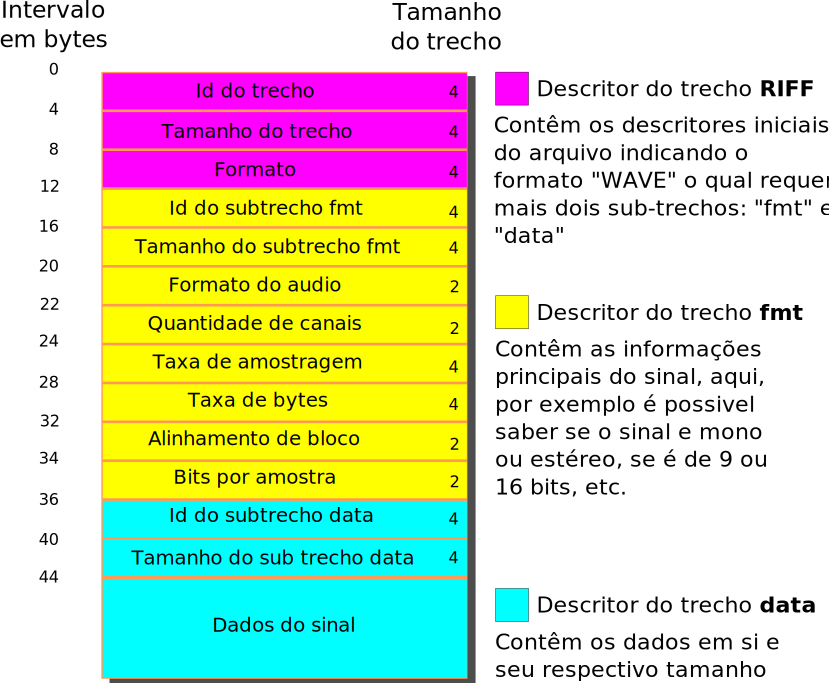
\includegraphics[width=.8\linewidth, angle=-90]{../monography/images/wavePcmStructure.pdf}
			\label{fig:wavePcmStructure}
		\end{figure}
		\column{0.4\textwidth}
		\begin{itemize}
			\item Formato \textit{wave}.
			\item \textit{Pulse-code modulation} (PCM).
			\item Taxa de amostragem de 44100hz.
			\item Resolução de 16bits
		\end{itemize}
	\end{columns}
\end{frame}
		\begin{frame}
	\frametitle{Sinais Digitais e Sub-amostragem (Downsampling)}
	\begin{figure}
		\centering
		\includegraphics[width=0.5\linewidth]{../monography/images/downsampling}
		\caption{Sub-amostragem}
		\label{fig:downsampling}
	\end{figure}
	\par Ocorre após a conversão de domínio dos sinais com base em filtros digitais do tipo \textit{wavelet}.
\end{frame}
		\begin{frame}
	\frametitle{Caracterização dos processos de produção da voz humana}
	\only<1>{
		\framesubtitle{Áreas de estudo}
		\begin{itemize}
			\item Fisiológica ou “fonética articulatória”.
			\item Acústica ou “fonética acústica”.
			\item Perceptual.
		\end{itemize}
		\textbf{Foco apenas na acústica}
	}
	\only<2>{
		\framesubtitle{Vozeada versus não-vozeada}
		\begin{itemize}
			\item Vozeada: Pregas vocais.
			\item Não vozeada: Sem pregas vocais.
		\end{itemize}
	}
	\only<3>{
		\framesubtitle{Frequência fundamental da voz}
		\begin{itemize}
			\item Conhecida como $F_0$.
			\item Componente periódico resultante da vibração das pregas vocais.
		\end{itemize}
	}
	\only<4>{
		\framesubtitle{Formantes}
		\begin{itemize}
			\item $F_1 \rightarrow$ amplificação  sonora  na  cavidade  oral  posterior,  posição  da  língua  no  plano  vertical.
			\item $F_2 \rightarrow$ cavidade  oral  anterior,  posição  da  língua  no  plano  horizontal.
			\item $F_3 \rightarrow$ cavidades  à  frente  e  atrás  do  ápice  da  língua.
			\item $F_4 \rightarrow$ formato da laringe e da  faringe.
		\end{itemize}
	}
\end{frame}
		\begin{frame}
	\frametitle{Distâncias Euclidiana e Manhattan}
	\begin{itemize}
		\item dsd
	\end{itemize}
\end{frame}


		\begin{frame}
	\frametitle{Bandas críticas de energia}
		\only<1>{
			\framesubtitle{Definições}
			\par Definem os intervalos em que serão calculadas as energias.\newline
			\begin{columns}
				\column{0.5\textwidth}
					\par A energia de um sinal digital $s[\cdot]$ com $M$ amostras é definida como
					\begin{equation}
						E = \sum\limits_{i=0}^{M-1}(s_i)^2 \qquad.   
					\end{equation}
				\column{0.5\textwidth}
					\begin{itemize}
						\item \textbf{BARK:} 20, 100, 200, 300, 400, 510, 630, 770, 920, 1080, 1270, 1480, 1720, 2000, 2320, 2700, 3150, 3700, 4400, 5300, 6400, 7700, 9500, 12000, 15500.
						\item \textbf{MEL:} 20, 160, 394, 670, 1000, 1420, 1900, 2450, 3120, 4000, 5100, 6600, 9000, 14000.
					\end{itemize}
			\end{columns}
		}
		\only<2>{
			\framesubtitle{Cálculo de vetores de características com BARK}
			\begin{figure}
				\centering
				\includegraphics[width=0.7\linewidth]{../monography/images/barkFeatureVect}
			\end{figure}
		}
		\only<3>{
			\framesubtitle{Cálculo de vetores de características com MEL}
			\begin{figure}
				\centering
				\includegraphics[width=0.5\linewidth]{../monography/images/melFeatureVect}
			\end{figure}
		}
\end{frame}
		\begin{frame}
	\frametitle{Filtros digitais \textit{wavelet}}
	\only<1>{
		\framesubtitle{Propriedades}
		\begin{itemize}
			\item Suporte compacto.
			\item Análise multirresolução.
			\item Wavelet regular e wavelet packet.
			\item Análise detalhada em altas e baixas frequências.
		\end{itemize}
	}
	\only<2>{
		\framesubtitle{Restrição de escopo}
		\begin{itemize}
			\item Domínio discreto.
			\item Apenas transformadas diretas.
			\item Não haverá reconstrução do sinal.
			\item Construção dos vetores de características.
		\end{itemize}
	}

	\only<3>{
		\framesubtitle{Resposta em frequência e linearidade}
		\begin{table}[h]
	\centering
	\caption{Algumas das \textit{wavelets} mais usadas e suas propriedades}
	\begin{tabular}{|c|p{75mm}|c|}
			\hline 
			\textbf{Wavelet} & \textbf{Resposta em frequência} & \textbf{Resposta em fase} \\ 
			\hline 
			Haar & Pobre &  Linear \\ 
			\hline 
			Daubechies & mais próxima da ideal à medida que o \newline  suporte aumenta; \textit{maximally-flat}  &  Não linear \\ 
			\hline 
			Symmlets & mais próxima da ideal à medida que o \newline  suporte aumenta; não \textit{maximally-flat}  & Quase linear \\ 
			\hline 
			Coiflets & mais próxima da ideal à medida que o \newline  suporte aumenta; não \textit{maximally-flat}  & Quase linear \\ 
			\hline 
	\end{tabular} 
	\label{tab:waveletsProperties}
	\\Fonte: Elaborado pelo autor, 2021.
\end{table}

	}

	\only<4>{
		\framesubtitle{Algoritmo de Malat}
		\begin{itemize}
			\item \textit{Wavelet} Haar: $h[\cdot] = [\frac{1}{\sqrt{2}}, \frac{1}{\sqrt{2}}]$.
			\item Par ortogonal: $g[\cdot] = [\frac{1}{\sqrt{2}}, \frac{-1}{\sqrt{2}}]$.
			\item sinal: $s[\cdot] = [1,2,3,4]$.
		\end{itemize}
		
		\begin{equation*}
			\begin{pmatrix}
			\frac{1}{\sqrt{2}}, \frac{1}{\sqrt{2}}, 0, 0\\
			\frac{1}{\sqrt{2}}, \frac{-1}{\sqrt{2}}, 0, 0\\
			0, 0, \frac{1}{\sqrt{2}}, \frac{1}{\sqrt{2}}\\
			0, 0, \frac{1}{\sqrt{2}}, \frac{1}{\sqrt{2}}\\
			\end{pmatrix} 
			\cdot
			\begin{pmatrix}
			1\\
			2\\
			3\\
			4\\
			\end{pmatrix} 
			=
			\begin{pmatrix}
			\frac{3}{\sqrt{2}}\\
			\frac{-1}{\sqrt{2}}\\
			\frac{7}{\sqrt{2}}\\
			\frac{-1}{\sqrt{2}}\\
			\end{pmatrix}
			\Rightarrow \Big[
			\frac{3}{\sqrt{2}},
			\frac{7}{\sqrt{2}},
			\frac{-1}{\sqrt{2}},
			\frac{-1}{\sqrt{2}}
			\Big]\qquad.
		\end{equation*}
	}

	\only<5>{
		\framesubtitle{Exemplo de wavelet regular e packet}
		\begin{figure}
			\centering
			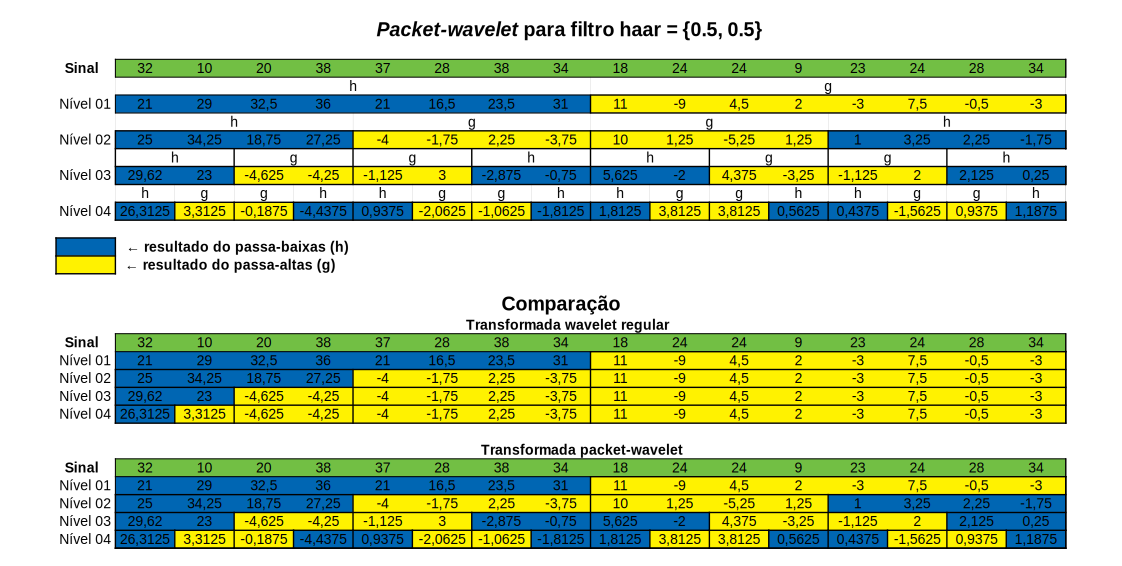
\includegraphics[width=\linewidth]{../monography/images/haarWaveletExamples}
		\end{figure}
	}
\end{frame}








		\begin{frame}
	\frametitle{Engenharia paraconsistente de características}
	\only<1>{
		\framesubtitle{Os vetores de características proporcionam uma boa separação interclasses?}
		\begin{columns}
		\column{.5\textwidth}				
		\begin{figure}
			\centering
			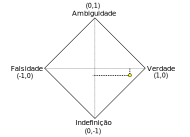
\includegraphics[width=.85\linewidth, angle=-90]{../monography/images/paraconsistentPlane}
			\label{fig:paraconsistentplane}
			\caption{Plano paraconsistente}
		\end{figure}
		\column{.5\textwidth}
		\begin{itemize}
			\item \alert{Verdade:\\
		 $\alpha = 1$ e $\beta = 0$.}
			\item Ambiguidade:\\
		 $\alpha = 1$ e $\beta = 1$.
			\item Falsidade:\\
		 $\alpha = 0$ e $\beta = 1$.
			\item Indefinição:\\
		 $\alpha = 0$ e $\beta = 0$.
		\end{itemize}
	\end{columns}
	}
	\only<2>{
		\framesubtitle{Cálculo de $\alpha$}
		\begin{columns}
			\column{.5\textwidth}
			\begin{textblock*}{0cm}(.4cm,1.5cm)
				\centering
				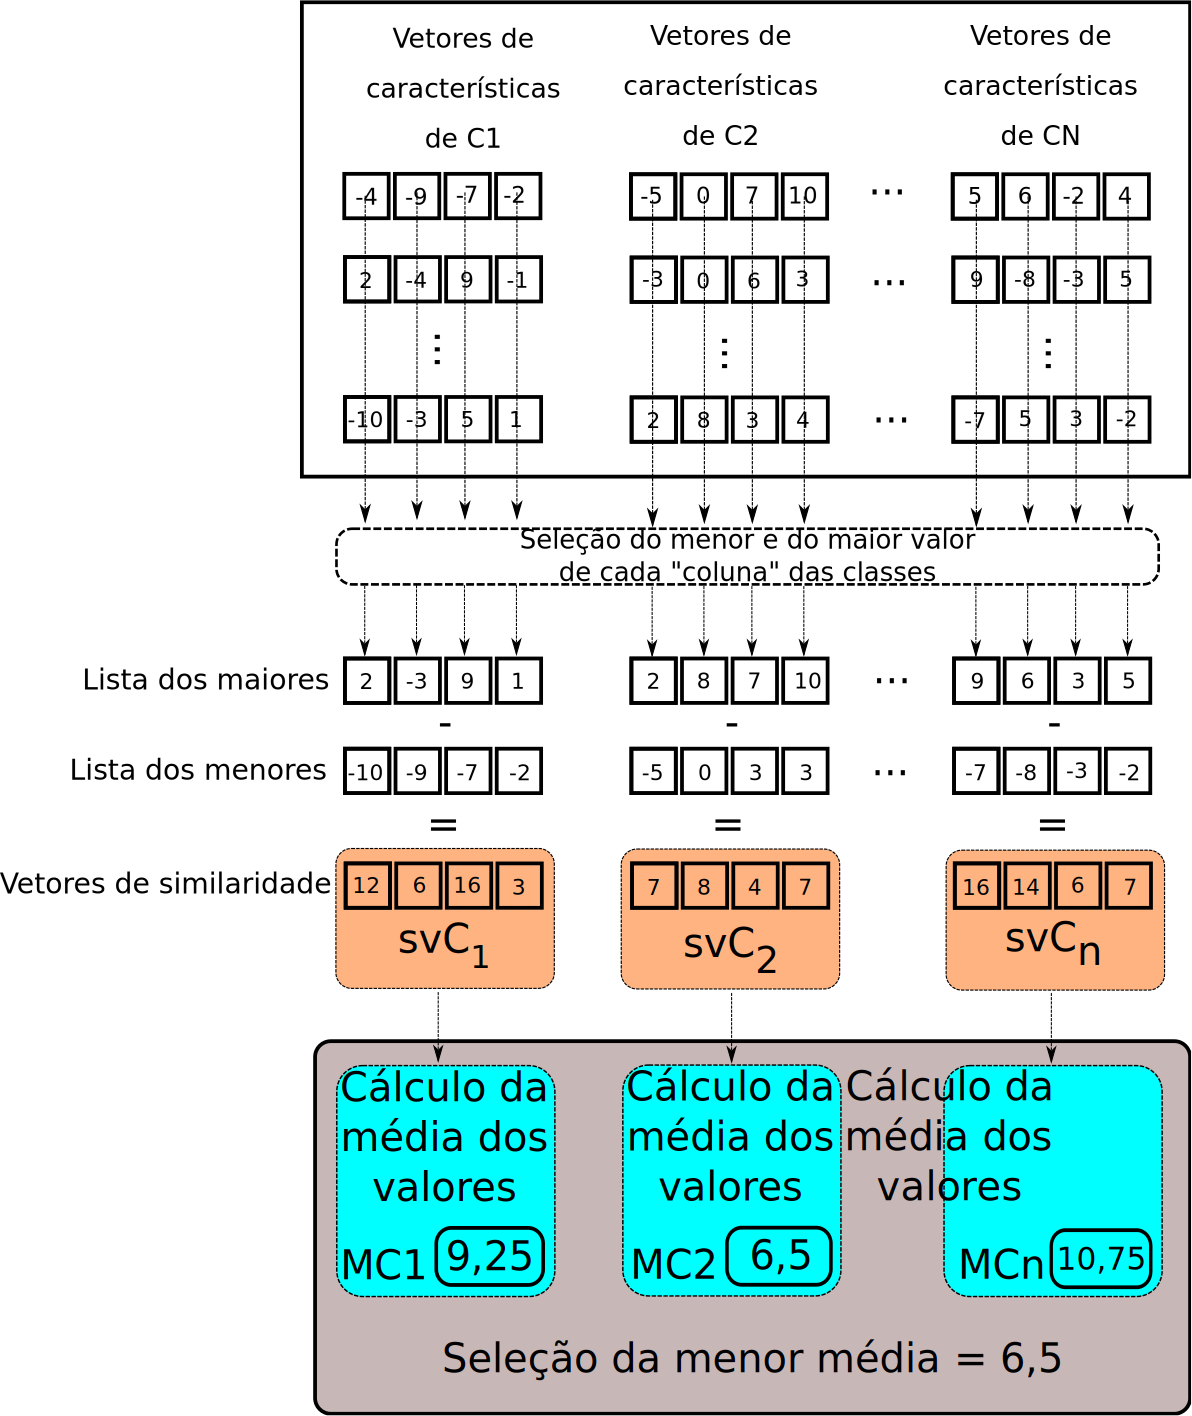
\includegraphics[height=0.82\textheight]{../monography/images/calculoAlpha.pdf}
			\end{textblock*}
			\column{.5\textwidth}
			\par Menor similaridade intraclasse, $\alpha$
		\end{columns}
	}
	\only<3>{
		\framesubtitle{Cálculo de $\beta$}
		\begin{columns}
			\column{.5\textwidth}
			\begin{textblock*}{0cm}(.4cm,1.5cm)
				\centering
				\includegraphics[height=.83\textheight]{../monography/images/betaCalculation.pdf}
			\end{textblock*}
			\column{.5\textwidth}
			\par Razão de sobreposição interclasse, $\beta$.
		\end{columns}
	}
	\only<4>{
		\framesubtitle{Graus de certeza e contradição}
		\begin{itemize}
			\item Grau de certeza $\rightarrow G_1=\alpha-\beta $.
			\item Grau de contradição $\rightarrow G_2=\alpha+\beta-1 $.				
		\end{itemize}
		Onde: $-1 \leqslant G_1 \leqslant 1$ e  $-1 \leqslant G_2 \leqslant 1\qquad$.\\
		Seja $P=(G_1,G_2)$
		\begin{itemize}
			\item (-1,0) $\rightarrow$ Falsidade;
			\item \alert{(1,0) $\rightarrow$ Verdade;}
			\item (0,-1) $\rightarrow$ Indefinição;
			\item (0,1) $\rightarrow$ Ambiguidade.
		\end{itemize}
	}
	\only<5>{
		\framesubtitle{Distancias no plano paraconsistente}
		As distâncias$(D)$ do ponto $P=(G_1,G_2)$ dos limites supracitados. Tal cálculo pode ser feito da seguinte forma:
		\begin{equation*}
		D_{-1,0}=\sqrt{(G_1+1)^2+(G_2)^2}\qquad,
		\end{equation*}
		\alert{
			\begin{equation*}
			D_{1,0}=\sqrt{(G_1-1)^2+(G_2)^2}\qquad,
			\end{equation*}
		}
		\begin{equation*}
		D_{0,-1}=\sqrt{(G_1)^2+(G_2+1)^2}\qquad,		
		\end{equation*}
		\begin{equation*}
		D_{0,1}=\sqrt{(G_1)^2+(G_2-1)^2}\qquad,
		\end{equation*}
	}
\end{frame}
	
	\section{Estado-da-arte em Playback Speech Detection}
		\begin{frame}[allowframebreaks]
	\frametitle{Trabalhos}
	\begin{itemize}
		\item \cite{Ren2019}: Energia e outras várias características do espectro do sinal, SVM.
		\item \cite{DiqunYan2019} \textit{Modelo oculto de Markov} (HMM); \textit{Wavelets}, SVM.
		\item \cite{7802552} \textit{Wavelets}, coeficientes cepstrais (SCCs), Modelos de mistura Gaussiana (GMM).
		\item \cite{alluri2019replay} \textit{"Zero time windowing"}(ZTW), análise cepstral do espectro GMM.
		\item \cite{8725688} Coeficientes cepstrais, GMM.
		\item \cite{Hanilci2018} Predição linear, coeficientes cepstrais, GMM.
		\item \cite{ISI:000473343500086} ``Texturas de voz'', padrões binários locais (LBP) e seus respectivos histogramas, SVM.
		\item Uma abordagem que combina análise de sinal de fala usando a \textit{Transformada Constante Q} (CQT) com o processamento cepstral foi mostrada no artigo \cite{TODISCO2017516}.
		\item No artigo \cite{Patel2015} é usada a \textit{Transformação Auditiva (TU)} que tem como base a transformada \textit{wavelet}, e a \textit{Cochlear Filter Cepstral Coefficients (CFCC)} juntamente com  \textit{estimação da frequência instantânea (IF)}.
		\item \cite{ISI:000490497200068} Partes não vozeadas da fala, três GMMs.
		\item \cite{ISI:000465363900136} amplitude instantânea vinda de flutuações de energia, GMM.
		\item \cite{ISI:000465363900139} Diferenças entre bandas de frequências específicas, \textit{predição linear em domínio de frequência}(FDLP), GMMs.
		\item \cite{Suthokumar2018} \textit{Modulation  spectral  centroid  frequency}, \textit{long term spectral average}, GMM.
		\item \cite{ISI:000458728700054} Envelopamento das amplitudes e das frequências instantâneas em cada banda estreita filtrada, GMM.
		\item \cite{ISI:000392503100008} \textit{Gammatone frequency cepstral coefficients}(MGFCC), GMM.
		\item \cite{8396208} \textit{Hashing} sensível a locus(LSH), MFCC e LSH, tabela \textit{hash}. 
	\end{itemize}
\end{frame}
\begin{frame}
	\frametitle{Comparativo}
		\begin{columns}
			\column{0.5\textwidth}
				\par \textbf{Referências}
				\begin{itemize}
					\item Apenas escala MEL.
					\item Classificadores simples.
					\item Uso escasso de wavelets.
					\item Uso do EER como métrica.
					\item Sem metodologia de seleção automática para os geradores de vetores de características.
				\end{itemize}
			\column{0.5\textwidth}
				\par \textbf{Dissertação}
				\begin{itemize}
					\item Escalas MEL e BARK.
					\item Classificadores simples.
					\item Uso intensivo wavelets.
					\item Uso de EER e acurácia como métrica.
					\item Seleção automática baseada na engenharia paraconsistente de características.
				\end{itemize}
		\end{columns}
\end{frame}
		
	\section{Contextualização}
		\begin{frame}
	\frametitle{Contextualização}
	\begin{itemize}
		\item Transformada \textit{Wavelet packet}: Boa resolução em relação às dimensões de tempo e frequência.
		\item Características mais disjuntas possíveis para de ``locutor autêntico'' e ``ataque de \textit{voice spoofing}''.
		\item Análise paraconsistente de acordo com o trabalho \cite{8588433}.
	\end{itemize}
\end{frame}

	\section{Abordagem proposta}
		\begin{frame}
	\frametitle{A Base de Sinais de Voz}
	\begin{itemize}
		\item 20 pessoas.
		\item Ambos sexos.
		\item Idades entre 7 e 60 anos.
		\item Dígitos falados de 0 a 9.
		\item Língua portuguesa e inglesa.
		\item Total de 820 sinais entre genuínos e regravados.
	\end{itemize}
\end{frame}
		\begin{frame}
	\frametitle{Estrutura da Estratégia Proposta}
	\begin{itemize}
		\item 
	\end{itemize}
\end{frame}
		\begin{frame}
	\frametitle{Procedimentos}
	\begin{itemize}
		\item 
	\end{itemize}
\end{frame}
		
	\section{Testes e Resultados}
		\begin{frame}
	\frametitle{Procedimento 01}
	\framesubtitle{Desempenho}
	\only<1>{
		\begin{itemize}
			\item Em se tratando das escalas, se verificou que BARK apresentou melhor desempenho em todas as combinações testadas.
			\item A combinação \textbf{\textit{wavelet} + Bark} apresentou, consistentemente, \textbf{melhor} viabilidade do que as respectivas combinações \textbf{\textit{wavelet + Mel}}.
			\item De todas as possibilidades verificadas a \textbf{\textit{wavelet} haar + Bark} apresentou o melhor desempenho.
		\end{itemize}
		
		\begin{table}
			\definecolor{tcB}{rgb}{0.447059,0.74902,0.266667}
			\definecolor{tcA}{rgb}{0.65098,0.65098,0.65098}
			\definecolor{tcC}{rgb}{1,0.94902,0}
			\centering
			\begin{tabular}{|c|c|c|c|}\hline
				% use packages: color,colortbl
				\rowcolor{tcA}
				Wavelet & G1 & G2 & Distância do ponto (1,0)\\\hline
				\rowcolor{tcB}
				haar & 0.93615 & 4.68316e-310 & 0.0638503\\\hline
				\multicolumn{1}{|>{\columncolor{tcC}}c|}{daub4} & \multicolumn{1}{>{\columncolor{tcC}}c|}{0.928088} & \multicolumn{1}{>{\columncolor{tcC}}c|}{4.68316e-310} & \multicolumn{1}{>{\columncolor{tcC}}c|}{0.0719123}\\\hline
				\multicolumn{1}{|>{\columncolor{tcC}}c|}{daub6} & \multicolumn{1}{>{\columncolor{tcC}}c|}{0.927885} & \multicolumn{1}{>{\columncolor{tcC}}c|}{4.68316e-310} & \multicolumn{1}{>{\columncolor{tcC}}c|}{0.072115}\\\hline
				\multicolumn{1}{|>{\columncolor{tcC}}c|}{coif6} & \multicolumn{1}{>{\columncolor{tcC}}c|}{0.927823} & \multicolumn{1}{>{\columncolor{tcC}}c|}{4.68316e-310} & \multicolumn{1}{>{\columncolor{tcC}}c|}{0.072177}\\\hline
				\multicolumn{1}{|>{\columncolor{tcC}}c|}{sym8} & \multicolumn{1}{>{\columncolor{tcC}}c|}{0.92769} & \multicolumn{1}{>{\columncolor{tcC}}c|}{4.68316e-310} & \multicolumn{1}{>{\columncolor{tcC}}c|}{0.0723096}\\\hline
				\multicolumn{1}{|>{\columncolor{tcC}}c|}{\tiny\vdots} & \multicolumn{1}{>{\columncolor{tcC}}c|}{\tiny\vdots} & \multicolumn{1}{>{\columncolor{tcC}}c|}{\tiny\vdots} & \multicolumn{1}{>{\columncolor{tcC}}c|}{\tiny\vdots}\\\hline
			\end{tabular}
		\end{table}
	}
	\only<2>{
		\begin{figure}
			\centering
			\includegraphics[width=0.7\linewidth]{images/results/paraconsistentPlane/ParaconsistentPart00}
			\caption{Quanto menor o comprimento horizontal das barras na cor azul, melhor a separabilidade entre as classes.}
		\end{figure}
	}
	
	\only<3>{
		\begin{figure}
			\centering
			\includegraphics[width=0.7\linewidth]{images/results/paraconsistentPlane/ParaconsistentPart01}
			\caption{Quanto menor o comprimento horizontal das barras na cor azul, melhor a separabilidade entre as classes.}
		\end{figure}
	}
	
	\only<4>{
		\begin{figure}
			\centering
			\includegraphics[width=0.7\linewidth]{images/results/paraconsistentPlane/ParaconsistentPart02}
			\caption{Quanto menor o comprimento horizontal das barras na cor azul, melhor a separabilidade entre as classes.}
		\end{figure}
	}
	
	\only<5>{
		\begin{figure}
			\centering
			\includegraphics[width=0.7\linewidth]{images/results/paraconsistentPlane/ParaconsistentPart03}
			\caption{Quanto menor o comprimento horizontal das barras na cor azul, melhor a separabilidade entre as classes.}
		\end{figure}
	}
	
	\only<6>{
		\framesubtitle{Síntese}
		\begin{columns}
			\column{0.5\textwidth}
			\begin{itemize}
				\item \textbf{Haar} e \textbf{Daubechies 42} proporcionaram, respectivamente, os melhores e os piores resultados associados com a escala Bark.
				\item Com a escala \textit{Mel}, \textbf{Haar} foi o melhor filtro e \textbf{Daubechies 54} o pior.
			\end{itemize}
			
			\par \textbf{\textit{Wavelet} Haar}
			\begin{itemize}
				\item Filtro de ordem 1
				\item Resposta perfeitamente linear.
				\item Contaminação por bandas adjacentes.
				\item Curva de resposta em frequência mais distante da ideal.
			\end{itemize}
			
			\column{0.5\textwidth}
			\par Portanto, experimentalmente, constatou-se que uma resposta em frequência não-rigorosa associada à uma resposta em fase perfeitamente linear é a melhor alternativa.\newline
			
			\par A \textbf{característica ruidosa} dos sinais regravados, contendo, ao contrário das vozes originais, notórios componentes de altas frequências, é melhor detectada com uma escala mais apropriada ao tratamento de áudio em geral e não voz somente.	
		\end{columns}
	}
	
\end{frame}
		\begin{frame}
	\frametitle{Procedimento 02}
	\framesubtitle{Descrição}
	\only<1>{
		\begin{itemize}
			\item 300 testes aleatórios em cada caso.
			\item EER = equilibrio entre as taxas de falsos positivos e de falsos negativos.
			\item Em alguns casos o cálculo do EER necessitou mais iterações.
			\item 10\%, 20\%, 30\%, 40\% e 50\% da base de sinais reservados para treinamento.
		\end{itemize}
	}	
\end{frame}
	
\begin{frame}[allowframebreaks]
	\frametitle{Procedimento 02}
		\framesubtitle{Tabelas de resultados}
		\begin{table}[H]
	\newcommand{\mc}[3]{\multicolumn{#1}{#2}{#3}}
	\definecolor{tcA}{rgb}{0.65098,0.65098,0.65098}
	\definecolor{tcB}{rgb}{0.447059,0.74902,0.266667}
	\begin{center}
		\begin{tabular}{|p{0.15\linewidth}|p{0.11\linewidth}|p{0.11\linewidth}|p{0.11\linewidth}|p{0.14\linewidth}|p{0.14\linewidth}|}\hline
			% use packages: color,colortbl
			\rowcolor{tcA}
			\centering\textbf{$M$} & \centering\textbf{Minimum value of accuracy} & \centering\textbf{Maximum value of accuracy} & \centering\textbf{Mean value of accuracy} & \centering\textbf{Standard deviation value of accuracy} & \textbf{\qquad EER}\\\hline

			\rowcolor{tcB}
			\mc{1}{|c|}{10\%} & \mc{1}{c|}{0.693767} & \mc{1}{c|}{0.867209} & \mc{1}{c|}{0.780488} & \mc{1}{c|}{0.021636} & \mc{1}{c|}{0.192412}\\\hline

			\rowcolor{tcB}
			\mc{1}{|c|}{20\%} & \mc{1}{c|}{0.734756} & \mc{1}{c|}{0.873476} & \mc{1}{c|}{0.804116} & \mc{1}{c|}{0.016209} & \mc{1}{c|}{0.182927}\\\hline

			\rowcolor{tcB}
			\mc{1}{|c|}{30\%} & \mc{1}{c|}{0.749129} & \mc{1}{c|}{0.881533} & \mc{1}{c|}{0.815331} & \mc{1}{c|}{0.014552} & \mc{1}{c|}{0.174216}\\\hline

			\rowcolor{tcB}
			\mc{1}{|c|}{40\%} & \mc{1}{c|}{0.760163} & \mc{1}{c|}{0.882114} & \mc{1}{c|}{0.8211385} & \mc{1}{c|}{0.014253} & \mc{1}{c|}{0.170732}\\\hline

			\rowcolor{tcB}
			\mc{1}{|c|}{50\%} & \mc{1}{c|}{0.756098} & \mc{1}{c|}{0.885366} & \mc{1}{c|}{0.820732} & \mc{1}{c|}{0.014974} & \mc{1}{c|}{0.165854}\\\hline
			
		\end{tabular}
	\end{center}
	\caption{Results for the pattern-matching approach and Euclidean distance.}
	\label{tab:experiment02ResultsEuclidian}
\end{table}

\begin{table}[H]
	\newcommand{\mc}[3]{\multicolumn{#1}{#2}{#3}}
	\definecolor{tcA}{rgb}{0.65098,0.65098,0.65098}
	\definecolor{tcB}{rgb}{0.447059,0.74902,0.266667}
	\begin{center}
		\begin{tabular}{|p{0.15\linewidth}|p{0.11\linewidth}|p{0.11\linewidth}|p{0.11\linewidth}|p{0.14\linewidth}|p{0.14\linewidth}|}\hline
			% use packages: color,colortbl
			\rowcolor{tcA}
			\centering\textbf{$M$} & \centering\textbf{Minimum value of accuracy} & \centering\textbf{Maximum value of accuracy} & \centering\textbf{Mean value of accuracy} & \centering\textbf{Standard deviation value of accuracy} & \textbf{\qquad EER}\\\hline
			
			\rowcolor{tcB}
			\mc{1}{|c|}{10\%} & \mc{1}{c|}{0.708672} & \mc{1}{c|}{0.878049} & \mc{1}{c|}{0.7933605} & \mc{1}{c|}{0.021617} & \mc{1}{c|}{0.184282}\\\hline

			\rowcolor{tcB}
			\mc{1}{|c|}{20\%} & \mc{1}{c|}{0.760671} & \mc{1}{c|}{0.885671} & \mc{1}{c|}{0.823171} & \mc{1}{c|}{0.0163} & \mc{1}{c|}{0.17378}\\\hline

			\rowcolor{tcB}
			\mc{1}{|c|}{30\%} & \mc{1}{c|}{0.768293} & \mc{1}{c|}{0.88676} & \mc{1}{c|}{0.8275265} & \mc{1}{c|}{0.01481} & \mc{1}{c|}{0.167247}\\\hline

			\rowcolor{tcB}
			\mc{1}{|c|}{40\%} & \mc{1}{c|}{0.778455} & \mc{1}{c|}{0.898374} & \mc{1}{c|}{0.8384145} & \mc{1}{c|}{0.014751} & \mc{1}{c|}{0.158537}\\\hline

			\rowcolor{tcB}
			\mc{1}{|c|}{50\%} & \mc{1}{c|}{0.778049} & \mc{1}{c|}{0.897561} & \mc{1}{c|}{0.837805} & \mc{1}{c|}{0.015646} & \mc{1}{c|}{0.156098}\\\hline		

		\end{tabular}
	\end{center}
	\caption{Results for the pattern-matching approach and Manhattan distance.}
	\label{tab:experiment02ResultsManhattan}
\end{table}
\end{frame}

\begin{frame}[allowframebreaks]
	\frametitle{Procedimento 02}
		\framesubtitle{Tabelas de confusão}
		\begin{table}[h] 					\newcommand{\mc}[3]{\multicolumn{#1}{#2}{#3}} 					\definecolor{tcB}{rgb}{0.447059,0.74902,0.266667} 					\definecolor{tcC}{rgb}{0,0,0} 					\definecolor{tcD}{rgb}{0,0.5,1} 					\definecolor{tcA}{rgb}{0.65098,0.65098,0.65098} 					\begin{center} 						\subfloat[Melhor matriz de confusão]{ 							\begin{tabular}{ccc} 								\mc{1}{l}{} & \mc{1}{>{\columncolor{tcA}}c}{\textbf{genuíno}} & \mc{1}{>{\columncolor{tcA}}c}{\textbf{falsificado}}\\ 								\mc{1}{>{\columncolor{tcA}}r}{\textbf{genuíno}} & \mc{1}{>{\columncolor{tcB}}c}{\textcolor{tcC}{363}} & \mc{1}{>{\columncolor{tcD}}c}{\textcolor{tcC}{14}}\\ 								\mc{1}{>{\columncolor{tcA}}r}{\textbf{falsificado}} & \mc{1}{>{\columncolor{tcD}}c}{\textcolor{tcC}{6}} & \mc{1}{>{\columncolor{tcB}}c}{\textcolor{tcC}{355}} 							\end{tabular} 							\label{tab:classifier_Euclidian_10_best} 						} 						\qquad 						\subfloat[Pior matriz de confusão]{ 							\begin{tabular}{ccc} 								\mc{1}{l}{} & \mc{1}{>{\columncolor{tcA}}c}{\textbf{genuíno}} & \mc{1}{>{\columncolor{tcA}}c}{\textbf{falsificado}}\\ 								\mc{1}{>{\columncolor{tcA}}r}{\textbf{genuíno}} & \mc{1}{>{\columncolor{tcB}}c}{\textcolor{tcC}{275}} & \mc{1}{>{\columncolor{tcD}}c}{\textcolor{tcC}{10}}\\ 								\mc{1}{>{\columncolor{tcA}}r}{\textbf{falsificado}} & \mc{1}{>{\columncolor{tcD}}c}{\textcolor{tcC}{94}} & \mc{1}{>{\columncolor{tcB}}c}{\textcolor{tcC}{359}} 							\end{tabular} 							\label{tab:classifier_Euclidian_10_worse} 						} 					\end{center} 					\caption{Matrizes de confusão para distância Euclidiana com modelo a 10\%} 				\end{table}
		\begin{table}[h]
\newcommand{\mc}[3]{\multicolumn{#1}{#2}{#3}}
\definecolor{tcB}{rgb}{0.447059,0.74902,0.266667}
\definecolor{tcC}{rgb}{0,0,0}
\definecolor{tcD}{rgb}{0,0.5,1}
\definecolor{tcA}{rgb}{0.65098,0.65098,0.65098}
\begin{center}
	\begin{tabular}{ccc}
		% use packages: color,colortbl
		\mc{1}{l}{} & \mc{1}{>{\columncolor{tcA}}c}{\textbf{genuine}} & \mc{1}{>{\columncolor{tcA}}c}{\textbf{spoofed}}\\

		\mc{1}{>{\columncolor{tcA}}r}{\textbf{genuine}} & \mc{1}{>{\columncolor{tcB}}c}{\textcolor{tcC}{308}} & \mc{1}{>{\columncolor{tcD}}c}{\textcolor{tcC}{50}}\\

		\mc{1}{>{\columncolor{tcA}}r}{\textbf{spoofed}} & \mc{1}{>{\columncolor{tcD}}c}{\textcolor{tcC}{20}} & \mc{1}{>{\columncolor{tcB}}c}{\textcolor{tcC}{278}}
	\end{tabular}
	\caption{Best confusion matrix for Euclidian distance classifier at 20\% model}
	\label{tab:classifier_Euclidian_20_best}
\end{center}
\end{table}

\begin{table}[h]
	\newcommand{\mc}[3]{\multicolumn{#1}{#2}{#3}}
	\definecolor{tcB}{rgb}{0.447059,0.74902,0.266667}
	\definecolor{tcC}{rgb}{0,0,0}
	\definecolor{tcD}{rgb}{0,0.5,1}
	\definecolor{tcA}{rgb}{0.65098,0.65098,0.65098}
	\begin{center}
		\begin{tabular}{ccc}
			% use packages: color,colortbl
			\mc{1}{l}{} & \mc{1}{>{\columncolor{tcA}}c}{\textbf{genuine}} & \mc{1}{>{\columncolor{tcA}}c}{\textbf{spoofed}}\\
			
			\mc{1}{>{\columncolor{tcA}}r}{\textbf{genuine}} & \mc{1}{>{\columncolor{tcB}}c}{\textcolor{tcC}{295}} & \mc{1}{>{\columncolor{tcD}}c}{\textcolor{tcC}{137}}\\
			
			\mc{1}{>{\columncolor{tcA}}r}{\textbf{spoofed}} & \mc{1}{>{\columncolor{tcD}}c}{\textcolor{tcC}{33}} & \mc{1}{>{\columncolor{tcB}}c}{\textcolor{tcC}{191}}
		\end{tabular}
		\caption{Worst confusion matrix for Euclidian distance classifier at 20\% model}
		\label{tab:classifier_Euclidian_20_worse}
	\end{center}
\end{table}

		\begin{table}[h] 					\newcommand{\mc}[3]{\multicolumn{#1}{#2}{#3}} 					\definecolor{tcB}{rgb}{0.447059,0.74902,0.266667} 					\definecolor{tcC}{rgb}{0,0,0} 					\definecolor{tcD}{rgb}{0,0.5,1} 					\definecolor{tcA}{rgb}{0.65098,0.65098,0.65098} 					\begin{center} 						\subfloat[Best confusion matrix]{ 							\begin{tabular}{ccc} 								\mc{1}{l}{} & \mc{1}{>{\columncolor{tcA}}c}{\textbf{genuine}} & \mc{1}{>{\columncolor{tcA}}c}{\textbf{spoofed}}\\ 								\mc{1}{>{\columncolor{tcA}}r}{\textbf{genuine}} & \mc{1}{>{\columncolor{tcB}}c}{\textcolor{tcC}{283}} & \mc{1}{>{\columncolor{tcD}}c}{\textcolor{tcC}{8}}\\ 								\mc{1}{>{\columncolor{tcA}}r}{\textbf{spoofed}} & \mc{1}{>{\columncolor{tcD}}c}{\textcolor{tcC}{4}} & \mc{1}{>{\columncolor{tcB}}c}{\textcolor{tcC}{279}} 							\end{tabular} 							\label{tab:classifier_Euclidian_30_best} 						} 						\qquad 						\subfloat[Worst confusion matrix]{ 							\begin{tabular}{ccc} 								\mc{1}{l}{} & \mc{1}{>{\columncolor{tcA}}c}{\textbf{genuine}} & \mc{1}{>{\columncolor{tcA}}c}{\textbf{spoofed}}\\ 								\mc{1}{>{\columncolor{tcA}}r}{\textbf{genuine}} & \mc{1}{>{\columncolor{tcB}}c}{\textcolor{tcC}{258}} & \mc{1}{>{\columncolor{tcD}}c}{\textcolor{tcC}{20}}\\ 								\mc{1}{>{\columncolor{tcA}}r}{\textbf{spoofed}} & \mc{1}{>{\columncolor{tcD}}c}{\textcolor{tcC}{29}} & \mc{1}{>{\columncolor{tcB}}c}{\textcolor{tcC}{267}} 							\end{tabular} 							\label{tab:classifier_Euclidian_30_worse} 						} 					\end{center} 					\caption{Confusion matrices for Euclidian distance classifier at 30\% model} 				\end{table}
		\begin{table}[h]
	\newcommand{\mc}[3]{\multicolumn{#1}{#2}{#3}}
	\definecolor{tcB}{rgb}{0.447059,0.74902,0.266667}
	\definecolor{tcC}{rgb}{0,0,0}
	\definecolor{tcD}{rgb}{0,0.5,1}
	\definecolor{tcA}{rgb}{0.65098,0.65098,0.65098}
	\begin{center}
		\subfloat[Melhor matriz]{
			\begin{tabular}{ccc}
				% use packages: color,colortbl
				\mc{1}{l}{} & \mc{1}{>{\columncolor{tcA}}c}{\textbf{genuíno}} & \mc{1}{>{\columncolor{tcA}}c}{\textbf{falseado}}\\
				
				\mc{1}{>{\columncolor{tcA}}r}{\textbf{genuíno}} & \mc{1}{>{\columncolor{tcB}}c}{\textcolor{tcC}{239}} & \mc{1}{>{\columncolor{tcD}}c}{\textcolor{tcC}{42}}\\
				
				\mc{1}{>{\columncolor{tcA}}r}{\textbf{falseado}} & \mc{1}{>{\columncolor{tcD}}c}{\textcolor{tcC}{7}} & \mc{1}{>{\columncolor{tcB}}c}{\textcolor{tcC}{204}}
			\end{tabular}
			\label{tab:classifier_Euclidian_40_best}
		}
		\qquad
		\subfloat[Pior matriz]{
			\begin{tabular}{ccc}
				% use packages: color,colortbl
				\mc{1}{l}{} & \mc{1}{>{\columncolor{tcA}}c}{\textbf{genuíno}} & \mc{1}{>{\columncolor{tcA}}c}{\textbf{falseado}}\\
				
				\mc{1}{>{\columncolor{tcA}}r}{\textbf{genuíno}} & \mc{1}{>{\columncolor{tcB}}c}{\textcolor{tcC}{232}} & \mc{1}{>{\columncolor{tcD}}c}{\textcolor{tcC}{99}}\\
				
				\mc{1}{>{\columncolor{tcA}}r}{\textbf{falseado}} & \mc{1}{>{\columncolor{tcD}}c}{\textcolor{tcC}{14}} & \mc{1}{>{\columncolor{tcB}}c}{\textcolor{tcC}{147}}
			\end{tabular}
			\label{tab:classifier_Euclidian_40_worse}
		}
	\end{center}
	\caption{Matrizes de confusão para o classificador por distâncias Euclidianas com o uso de 40\% da base para modelagem}
\end{table}

		\begin{table}[H] 					\newcommand{\mc}[3]{\multicolumn{#1}{#2}{#3}} 					\definecolor{tcB}{rgb}{0.447059,0.74902,0.266667} 					\definecolor{tcC}{rgb}{0,0,0} 					\definecolor{tcD}{rgb}{0,0.5,1} 					\definecolor{tcA}{rgb}{0.65098,0.65098,0.65098} 					\begin{center} 						\subfloat[Best confusion matrix]{ 							\begin{tabular}{ccc} 								\mc{1}{l}{} & \mc{1}{>{\columncolor{tcA}}c}{\textbf{genuine}} & \mc{1}{>{\columncolor{tcA}}c}{\textbf{spoofed}}\\ 								\mc{1}{>{\columncolor{tcA}}r}{\textbf{genuine}} & \mc{1}{>{\columncolor{tcB}}c}{\textcolor{tcC}{177}} & \mc{1}{>{\columncolor{tcD}}c}{\textcolor{tcC}{19}}\\ 								\mc{1}{>{\columncolor{tcA}}r}{\textbf{spoofed}} & \mc{1}{>{\columncolor{tcD}}c}{\textcolor{tcC}{28}} & \mc{1}{>{\columncolor{tcB}}c}{\textcolor{tcC}{186}} 							\end{tabular} 							\label{tab:classifier_Euclidian_50_best} 						} 						\qquad 						\subfloat[Worst confusion matrix]{ 							\begin{tabular}{ccc} 								\mc{1}{l}{} & \mc{1}{>{\columncolor{tcA}}c}{\textbf{genuine}} & \mc{1}{>{\columncolor{tcA}}c}{\textbf{spoofed}}\\ 								\mc{1}{>{\columncolor{tcA}}r}{\textbf{genuine}} & \mc{1}{>{\columncolor{tcB}}c}{\textcolor{tcC}{149}} & \mc{1}{>{\columncolor{tcD}}c}{\textcolor{tcC}{44}}\\ 								\mc{1}{>{\columncolor{tcA}}r}{\textbf{spoofed}} & \mc{1}{>{\columncolor{tcD}}c}{\textcolor{tcC}{56}} & \mc{1}{>{\columncolor{tcB}}c}{\textcolor{tcC}{161}} 							\end{tabular} 							\label{tab:classifier_Euclidian_50_worse} 						} 					\end{center} 					\caption{Confusion matrices for Euclidian distance classifier at 50\% model} 				\end{table}
		\begin{table}[h] 					\newcommand{\mc}[3]{\multicolumn{#1}{#2}{#3}} 					\definecolor{tcB}{rgb}{0.447059,0.74902,0.266667} 					\definecolor{tcC}{rgb}{0,0,0} 					\definecolor{tcD}{rgb}{0,0.5,1} 					\definecolor{tcA}{rgb}{0.65098,0.65098,0.65098} 					\begin{center} 						\subfloat[Melhor matriz de confusão]{ 							\begin{tabular}{ccc} 								\mc{1}{l}{} & \mc{1}{>{\columncolor{tcA}}c}{\textbf{genuíno}} & \mc{1}{>{\columncolor{tcA}}c}{\textbf{falsificado}}\\ 								\mc{1}{>{\columncolor{tcA}}r}{\textbf{genuíno}} & \mc{1}{>{\columncolor{tcB}}c}{\textcolor{tcC}{365}} & \mc{1}{>{\columncolor{tcD}}c}{\textcolor{tcC}{14}}\\ 								\mc{1}{>{\columncolor{tcA}}r}{\textbf{falsificado}} & \mc{1}{>{\columncolor{tcD}}c}{\textcolor{tcC}{4}} & \mc{1}{>{\columncolor{tcB}}c}{\textcolor{tcC}{355}} 							\end{tabular} 							\label{tab:classifier_Manhattan_10_best} 						} 						\qquad 						\subfloat[Pior matriz de confusão]{ 							\begin{tabular}{ccc} 								\mc{1}{l}{} & \mc{1}{>{\columncolor{tcA}}c}{\textbf{genuíno}} & \mc{1}{>{\columncolor{tcA}}c}{\textbf{falsificado}}\\ 								\mc{1}{>{\columncolor{tcA}}r}{\textbf{genuíno}} & \mc{1}{>{\columncolor{tcB}}c}{\textcolor{tcC}{289}} & \mc{1}{>{\columncolor{tcD}}c}{\textcolor{tcC}{11}}\\ 								\mc{1}{>{\columncolor{tcA}}r}{\textbf{falsificado}} & \mc{1}{>{\columncolor{tcD}}c}{\textcolor{tcC}{80}} & \mc{1}{>{\columncolor{tcB}}c}{\textcolor{tcC}{358}} 							\end{tabular} 							\label{tab:classifier_Manhattan_10_worse} 						} 					\end{center} 					\caption{Matrizes de confusão para distância Manhattan com modelo a 10\%} 				\end{table}
		\begin{table}[h]
\newcommand{\mc}[3]{\multicolumn{#1}{#2}{#3}}
\definecolor{tcB}{rgb}{0.447059,0.74902,0.266667}
\definecolor{tcC}{rgb}{0,0,0}
\definecolor{tcD}{rgb}{0,0.5,1}
\definecolor{tcA}{rgb}{0.65098,0.65098,0.65098}
\begin{center}
	\begin{tabular}{ccc}
		% use packages: color,colortbl
		\mc{1}{l}{} & \mc{1}{>{\columncolor{tcA}}c}{\textbf{Verdadeiro}} & \mc{1}{>{\columncolor{tcA}}c}{\textbf{Falso}}\\

		\mc{1}{>{\columncolor{tcA}}r}{\textbf{Verdadeiro}} & \mc{1}{>{\columncolor{tcB}}c}{\textcolor{tcC}{308}} & \mc{1}{>{\columncolor{tcD}}c}{\textcolor{tcC}{44}}\\

		\mc{1}{>{\columncolor{tcA}}r}{\textbf{Falso}} & \mc{1}{>{\columncolor{tcD}}c}{\textcolor{tcC}{20}} & \mc{1}{>{\columncolor{tcB}}c}{\textcolor{tcC}{284}}
	\end{tabular}
	\caption{Matriz de confusão para o classificador por distâncias Manhattan com o uso de 20\% da base para modelagem}
	\label{tab:classifier_Manhattan_20_best}
\end{center}
\end{table}

\begin{table}[h]
	\newcommand{\mc}[3]{\multicolumn{#1}{#2}{#3}}
	\definecolor{tcB}{rgb}{0.447059,0.74902,0.266667}
	\definecolor{tcC}{rgb}{0,0,0}
	\definecolor{tcD}{rgb}{0,0.5,1}
	\definecolor{tcA}{rgb}{0.65098,0.65098,0.65098}
	\begin{center}
		\begin{tabular}{ccc}
			% use packages: color,colortbl
			\mc{1}{l}{} & \mc{1}{>{\columncolor{tcA}}c}{\textbf{Verdadeiro}} & \mc{1}{>{\columncolor{tcA}}c}{\textbf{Falso}}\\
			
			\mc{1}{>{\columncolor{tcA}}r}{\textbf{Verdadeiro}} & \mc{1}{>{\columncolor{tcB}}c}{\textcolor{tcC}{316}} & \mc{1}{>{\columncolor{tcD}}c}{\textcolor{tcC}{149}}\\
			
			\mc{1}{>{\columncolor{tcA}}r}{\textbf{Falso}} & \mc{1}{>{\columncolor{tcD}}c}{\textcolor{tcC}{12}} & \mc{1}{>{\columncolor{tcB}}c}{\textcolor{tcC}{179}}
		\end{tabular}
		\caption{Pior matriz de confusão para o classificador por distâncias Manhattan com o uso de 20\% da base para modelagem}
		\label{tab:classifier_Manhattan_20_worst}
	\end{center}
\end{table}

		\begin{table}[h]
	\newcommand{\mc}[3]{\multicolumn{#1}{#2}{#3}}
	\definecolor{tcB}{rgb}{0.447059,0.74902,0.266667}
	\definecolor{tcC}{rgb}{0,0,0}
	\definecolor{tcD}{rgb}{0,0.5,1}
	\definecolor{tcA}{rgb}{0.65098,0.65098,0.65098}
	\begin{center}
		\subfloat[Best matrix]{
			\begin{tabular}{ccc}
				% use packages: color,colortbl
				\mc{1}{l}{} & \mc{1}{>{\columncolor{tcA}}c}{\textbf{genuine}} & \mc{1}{>{\columncolor{tcA}}c}{\textbf{spoofed}}\\
				
				\mc{1}{>{\columncolor{tcA}}r}{\textbf{genuine}} & \mc{1}{>{\columncolor{tcB}}c}{\textcolor{tcC}{276}} & \mc{1}{>{\columncolor{tcD}}c}{\textcolor{tcC}{44}}\\
				
				\mc{1}{>{\columncolor{tcA}}r}{\textbf{spoofed}} & \mc{1}{>{\columncolor{tcD}}c}{\textcolor{tcC}{11}} & \mc{1}{>{\columncolor{tcB}}c}{\textcolor{tcC}{243}}
			\end{tabular}
			\label{tab:classifier_Manhattan_30_best}
		}
		\qquad
		\subfloat[Worst matrix]{
			\begin{tabular}{ccc}
				% use packages: color,colortbl
				\mc{1}{l}{} & \mc{1}{>{\columncolor{tcA}}c}{\textbf{genuine}} & \mc{1}{>{\columncolor{tcA}}c}{\textbf{spoofed}}\\
				
				\mc{1}{>{\columncolor{tcA}}r}{\textbf{genuine}} & \mc{1}{>{\columncolor{tcB}}c}{\textcolor{tcC}{266}} & \mc{1}{>{\columncolor{tcD}}c}{\textcolor{tcC}{106}}\\
				
				\mc{1}{>{\columncolor{tcA}}r}{\textbf{spoofed}} & \mc{1}{>{\columncolor{tcD}}c}{\textcolor{tcC}{21}} & \mc{1}{>{\columncolor{tcB}}c}{\textcolor{tcC}{181}}
			\end{tabular}
			\label{tab:classifier_Manhattan_30_worse}
		}
	\end{center}
	\caption{Confusion matrices for Manhattan distance classifier at 30\% model}
\end{table}
		\begin{table}[h]
	\newcommand{\mc}[3]{\multicolumn{#1}{#2}{#3}}
	\definecolor{tcB}{rgb}{0.447059,0.74902,0.266667}
	\definecolor{tcC}{rgb}{0,0,0}
	\definecolor{tcD}{rgb}{0,0.5,1}
	\definecolor{tcA}{rgb}{0.65098,0.65098,0.65098}
	\begin{center}
		\subfloat[Melhor matriz]{
			\begin{tabular}{ccc}
				% use packages: color,colortbl
				\mc{1}{l}{} & \mc{1}{>{\columncolor{tcA}}c}{\textbf{Verdadeiro}} & \mc{1}{>{\columncolor{tcA}}c}{\textbf{Falso}}\\
				
				\mc{1}{>{\columncolor{tcA}}r}{\textbf{Verdadeiro}} & \mc{1}{>{\columncolor{tcB}}c}{\textcolor{tcC}{239}} & \mc{1}{>{\columncolor{tcD}}c}{\textcolor{tcC}{41}}\\
				
				\mc{1}{>{\columncolor{tcA}}r}{\textbf{Falso}} & \mc{1}{>{\columncolor{tcD}}c}{\textcolor{tcC}{7}} & \mc{1}{>{\columncolor{tcB}}c}{\textcolor{tcC}{205}}
			\end{tabular}
			\label{tab:classifier_Manhattan_40_best}
		}
		\qquad
		\subfloat[Pior matriz]{
			\begin{tabular}{ccc}
				% use packages: color,colortbl
				\mc{1}{l}{} & \mc{1}{>{\columncolor{tcA}}c}{\textbf{Verdadeiro}} & \mc{1}{>{\columncolor{tcA}}c}{\textbf{Falso}}\\
				
				\mc{1}{>{\columncolor{tcA}}r}{\textbf{Verdadeiro}} & \mc{1}{>{\columncolor{tcB}}c}{\textcolor{tcC}{227}} & \mc{1}{>{\columncolor{tcD}}c}{\textcolor{tcC}{91}}\\
				
				\mc{1}{>{\columncolor{tcA}}r}{\textbf{Falso}} & \mc{1}{>{\columncolor{tcD}}c}{\textcolor{tcC}{19}} & \mc{1}{>{\columncolor{tcB}}c}{\textcolor{tcC}{155}}
			\end{tabular}
			\label{tab:classifier_Manhattan_40_worse}
		}
	\end{center}
	\caption{Matrizes de confusão para o classificador por distâncias Manhattan com o uso de 40\% da base para modelagem}
\end{table}

		\begin{table}[H] 					\newcommand{\mc}[3]{\multicolumn{#1}{#2}{#3}} 					\definecolor{tcB}{rgb}{0.447059,0.74902,0.266667} 					\definecolor{tcC}{rgb}{0,0,0} 					\definecolor{tcD}{rgb}{0,0.5,1} 					\definecolor{tcA}{rgb}{0.65098,0.65098,0.65098} 					\begin{center} 						\subfloat[Melhor matriz de confusão]{ 							\begin{tabular}{ccc} 								\mc{1}{l}{} & \mc{1}{>{\columncolor{tcA}}c}{\textbf{genuíno}} & \mc{1}{>{\columncolor{tcA}}c}{\textbf{falseado}}\\ 								\mc{1}{>{\columncolor{tcA}}r}{\textbf{genuíno}} & \mc{1}{>{\columncolor{tcB}}c}{\textcolor{tcC}{203}} & \mc{1}{>{\columncolor{tcD}}c}{\textcolor{tcC}{2}}\\ 								\mc{1}{>{\columncolor{tcA}}r}{\textbf{falseado}} & \mc{1}{>{\columncolor{tcD}}c}{\textcolor{tcC}{2}} & \mc{1}{>{\columncolor{tcB}}c}{\textcolor{tcC}{203}} 							\end{tabular} 							\label{tab:classifier_Manhattan_50_best} 						} 						\qquad 						\subfloat[Pior matriz de confusão]{ 							\begin{tabular}{ccc} 								\mc{1}{l}{} & \mc{1}{>{\columncolor{tcA}}c}{\textbf{genuíno}} & \mc{1}{>{\columncolor{tcA}}c}{\textbf{falseado}}\\ 								\mc{1}{>{\columncolor{tcA}}r}{\textbf{genuíno}} & \mc{1}{>{\columncolor{tcB}}c}{\textcolor{tcC}{188}} & \mc{1}{>{\columncolor{tcD}}c}{\textcolor{tcC}{13}}\\ 								\mc{1}{>{\columncolor{tcA}}r}{\textbf{falseado}} & \mc{1}{>{\columncolor{tcD}}c}{\textcolor{tcC}{17}} & \mc{1}{>{\columncolor{tcB}}c}{\textcolor{tcC}{192}} 							\end{tabular} 							\label{tab:classifier_Manhattan_50_worse} 						} 					\end{center} 					\caption{Matrizes de confusão para distância Manhattan com modelo a 50\%} 				\end{table}
\end{frame}
	
\begin{frame}
	\frametitle{Procedimento 02}
	\framesubtitle{Acurácias e EER para distância Euclidiana}
	\only<1>{
		\begin{columns}
			\column{0.5\textwidth}
			\begin{figure}
				\centering
				\includegraphics[width=\linewidth]{../monography/images/results/confusionMatrices/classifier_Euclidian_10}
				\caption{Acurácia \textit{X} quantidade de testes - Distância Euclidiana, modelo a 10\%}
			\end{figure}
			
			\column{0.5\textwidth}
			\begin{figure}
				\centering
				\includegraphics[width=\linewidth]{../monography/images/results/det/DET_for_classifier_Euclidian_10}
				\caption{Curva DET dos resultados de distância Euclidiana, modelo a 10\%}
			\end{figure}
		\end{columns}
	}
	\only<2>{
		\begin{columns}
			\column{0.5\textwidth}
			\begin{figure}
				\centering
				\includegraphics[width=\linewidth]{../monography/images/results/confusionMatrices/classifier_Euclidian_20}
				\caption{Acurácia \textit{X} quantidade de testes - Distância Euclidiana, modelo a 20\%}
			\end{figure}
			
			\column{0.5\textwidth}
			\begin{figure}
				\centering
				\includegraphics[width=\linewidth]{../monography/images/results/det/DET_for_classifier_Euclidian_20}
				\caption{Curva DET dos resultados de distância Euclidiana, modelo a 20\%}
			\end{figure}
		\end{columns}
	}
	\only<3>{
		\begin{columns}
			\column{0.5\textwidth}
			\begin{figure}
				\centering
				\includegraphics[width=\linewidth]{../monography/images/results/confusionMatrices/classifier_Euclidian_30}
				\caption{Acurácia \textit{X} quantidade de testes - Distância Euclidiana, modelo a 30\%}
			\end{figure}
			
			\column{0.5\textwidth}
			\begin{figure}
				\centering
				\includegraphics[width=\linewidth]{../monography/images/results/det/DET_for_classifier_Euclidian_30}
				\caption{Curva DET dos resultados de distância Euclidiana, modelo a 30\%}
			\end{figure}
		\end{columns}
	}
	\only<4>{
		\begin{columns}
			\column{0.5\textwidth}
			\begin{figure}
				\centering
				\includegraphics[width=\linewidth]{../monography/images/results/confusionMatrices/classifier_Euclidian_40}
				\caption{Acurácia \textit{X} quantidade de testes - Distância Euclidiana, modelo a 40\%}
			\end{figure}
			
			\column{0.5\textwidth}
			\begin{figure}
				\centering
				\includegraphics[width=\linewidth]{../monography/images/results/det/DET_for_classifier_Euclidian_40}
				\caption{Curva DET dos resultados de distância Euclidiana, modelo a 40\%}
			\end{figure}
		\end{columns}
	}
	\only<5>{
		\begin{columns}
			\column{0.5\textwidth}
			\begin{figure}
				\centering
				\includegraphics[width=\linewidth]{../monography/images/results/confusionMatrices/classifier_Euclidian_50}
				\caption{Acurácia \textit{X} quantidade de testes - Distância Euclidiana, modelo a 50\%}
			\end{figure}
			
			\column{0.5\textwidth}
			\begin{figure}
				\centering
				\includegraphics[width=\linewidth]{../monography/images/results/det/DET_for_classifier_Euclidian_50}
				\caption{Curva DET dos resultados de distância Euclidiana, modelo a 50\%}
			\end{figure}
		\end{columns}
	}
\end{frame}

\begin{frame}
	\frametitle{Procedimento 02}
	\framesubtitle{Acurácias e EER para distância Manhattan}
	\only<1>{
		\begin{columns}
			\column{0.5\textwidth}
			\begin{figure}
				\centering
				\includegraphics[width=\linewidth]{../monography/images/results/confusionMatrices/classifier_Manhattan_10}
				\caption{Acurácia \textit{X} quantidade de testes - Distância Manhattan, modelo a 10\%}
			\end{figure}
			
			\column{0.5\textwidth}
			\begin{figure}
				\centering
				\includegraphics[width=\linewidth]{../monography/images/results/det/DET_for_classifier_Manhattan_10}
				\caption{Curva DET dos resultados de distância Manhattan, modelo a 10\%}
			\end{figure}
		\end{columns}
	}
	\only<2>{
		\begin{columns}
			\column{0.5\textwidth}
			\begin{figure}
				\centering
				\includegraphics[width=\linewidth]{../monography/images/results/confusionMatrices/classifier_Manhattan_20}
				\caption{Acurácia \textit{X} quantidade de testes - Distância Manhattan, modelo a 20\%}
			\end{figure}
			
			\column{0.5\textwidth}
			\begin{figure}
				\centering
				\includegraphics[width=\linewidth]{../monography/images/results/det/DET_for_classifier_Manhattan_20}
				\caption{Curva DET dos resultados de distância Manhattan, modelo a 20\%}
			\end{figure}
		\end{columns}
	}
	\only<3>{
		\begin{columns}
			\column{0.5\textwidth}
			\begin{figure}
				\centering
				\includegraphics[width=\linewidth]{../monography/images/results/confusionMatrices/classifier_Manhattan_30}
				\caption{Acurácia \textit{X} quantidade de testes - Distância Manhattan, modelo a 30\%}
			\end{figure}
			
			\column{0.5\textwidth}
			\begin{figure}
				\centering
				\includegraphics[width=\linewidth]{../monography/images/results/det/DET_for_classifier_Manhattan_30}
				\caption{Curva DET dos resultados de distância Manhattan, modelo a 30\%}
			\end{figure}
		\end{columns}
	}
	\only<4>{
		\begin{columns}
			\column{0.5\textwidth}
			\begin{figure}
				\centering
				\includegraphics[width=\linewidth]{../monography/images/results/confusionMatrices/classifier_Manhattan_40}
				\caption{Acurácia \textit{X} quantidade de testes - Distância Manhattan, modelo a 40\%}
			\end{figure}
			
			\column{0.5\textwidth}
			\begin{figure}
				\centering
				\includegraphics[width=\linewidth]{../monography/images/results/det/DET_for_classifier_Manhattan_40}
				\caption{Curva DET dos resultados de distância Manhattan, modelo a 40\%}
			\end{figure}
		\end{columns}
	}
	\only<5>{
		\begin{columns}
			\column{0.5\textwidth}
			\begin{figure}
				\centering
				\includegraphics[width=\linewidth]{../monography/images/results/confusionMatrices/classifier_Manhattan_50}
				\caption{Acurácia \textit{X} quantidade de testes - Distância Manhattan, modelo a 50\%}
			\end{figure}
			
			\column{0.5\textwidth}
			\begin{figure}
				\centering
				\includegraphics[width=\linewidth]{../monography/images/results/det/DET_for_classifier_Manhattan_50}
				\caption{Curva DET dos resultados de distância Manhattan, modelo a 50\%}
			\end{figure}
		\end{columns}
	}
\end{frame}

\begin{frame}
	\frametitle{Procedimento 02}
		\framesubtitle{Síntese}
		\par Dentre os testes realizados o melhores resultados foram:
		\begin{itemize}
			\item Distância Euclidiana $\rightarrow$ Acurácia: 0,987805 - ERR: 0,039024.
			\item Distância Manhattan $\rightarrow$ Acurácia: 0,990244 - ERR: 0,039024.
		\end{itemize}
\end{frame}
		\begin{frame}
	\frametitle{Procedimento 03}
	\framesubtitle{Descrição}
	\only<1>{
		\begin{itemize}
			\item 300 testes aleatórios em cada caso.
			\item EER = equilibrio entre as taxas de falsos positivos e de falsos negativos.
			\item Em alguns casos o cálculo do EER necessitou mais iterações.
			\item 10\%, 20\%, 30\%, 40\% e 50\% da base de sinais reservados para treinamento.
		\end{itemize}
	}	
\end{frame}

\begin{frame}
	\frametitle{Procedimento 03}
	\framesubtitle{Tabela de resultados}
	\begin{table}[H]
	\newcommand{\mc}[3]{\multicolumn{#1}{#2}{#3}}
	\definecolor{tcA}{rgb}{0.65098,0.65098,0.65098}
	\definecolor{tcB}{rgb}{0.447059,0.74902,0.266667}
	\begin{center}
		\begin{tabular}{|p{0.15\linewidth}|p{0.11\linewidth}|p{0.11\linewidth}|p{0.18\linewidth}|p{0.2\linewidth}|p{0.11\linewidth}|}\hline
			% use packages: color,colortbl
			\rowcolor{tcA}
			\centering\textbf{M} & \centering\textbf{Minimum accuracy} & \centering\textbf{Maximum accuracy} & \centering\textbf{Mean of accuracies} &  \centering\textbf{Standard deviation of accuracies} & \textbf{\space \space \space EER}\\\hline
			\rowcolor{tcB}\mc{1}{|c|}{10\%} & \mc{1}{c|}{0.776423} & \mc{1}{c|}{0.911924} & \mc{1}{c|}{0.8441735} & \mc{1}{c|}{0.014714} & \mc{1}{c|}{0.199187}\\\hline
			\rowcolor{tcB}\mc{1}{|c|}{20\%} & \mc{1}{c|}{0.815549} & \mc{1}{c|}{0.919207} & \mc{1}{c|}{0.867378 } & \mc{1}{c|}{0.010975} & \mc{1}{c|}{0.185976}\\\hline
			\rowcolor{tcB}\mc{1}{|c|}{30\%} & \mc{1}{c|}{0.841463} & \mc{1}{c|}{0.926829} & \mc{1}{c|}{0.884146 } & \mc{1}{c|}{0.010565} & \mc{1}{c|}{0.1777  }\\\hline
			\rowcolor{tcB}\mc{1}{|c|}{40\%} & \mc{1}{c|}{0.841463} & \mc{1}{c|}{0.939024} & \mc{1}{c|}{0.8902435} & \mc{1}{c|}{0.01102 } & \mc{1}{c|}{0.170732}\\\hline
			\rowcolor{tcB}\mc{1}{|c|}{50\%} & \mc{1}{c|}{0.836585} & \mc{1}{c|}{0.939024} & \mc{1}{c|}{0.8878045} & \mc{1}{c|}{0.012119} & \mc{1}{c|}{0.170732}\\\hline		
		\end{tabular}
	\end{center}
	\caption{Procedure 03 results}
	\label{tab:experiment03Results}
\end{table}
\end{frame}

\begin{frame}[allowframebreaks]
	\frametitle{Procedimento 03}
	\framesubtitle{Tabelas de confusão}
	\begin{table}[h] 					\newcommand{\mc}[3]{\multicolumn{#1}{#2}{#3}} 					\definecolor{tcB}{rgb}{0.447059,0.74902,0.266667} 					\definecolor{tcC}{rgb}{0,0,0} 					\definecolor{tcD}{rgb}{0,0.5,1} 					\definecolor{tcA}{rgb}{0.65098,0.65098,0.65098} 					\begin{center} 						\subfloat[Melhor matriz de confusão]{ 							\begin{tabular}{ccc} 								\mc{1}{l}{} & \mc{1}{>{\columncolor{tcA}}c}{\textbf{genuíno}} & \mc{1}{>{\columncolor{tcA}}c}{\textbf{falsificado}}\\ 								\mc{1}{>{\columncolor{tcA}}r}{\textbf{genuíno}} & \mc{1}{>{\columncolor{tcB}}c}{\textcolor{tcC}{366}} & \mc{1}{>{\columncolor{tcD}}c}{\textcolor{tcC}{10}}\\ 								\mc{1}{>{\columncolor{tcA}}r}{\textbf{falsificado}} & \mc{1}{>{\columncolor{tcD}}c}{\textcolor{tcC}{3}} & \mc{1}{>{\columncolor{tcB}}c}{\textcolor{tcC}{359}} 							\end{tabular} 							\label{tab:classifier_SVM_10_best} 						} 						\qquad 						\subfloat[Pior matriz de confusão]{ 							\begin{tabular}{ccc} 								\mc{1}{l}{} & \mc{1}{>{\columncolor{tcA}}c}{\textbf{genuíno}} & \mc{1}{>{\columncolor{tcA}}c}{\textbf{falsificado}}\\ 								\mc{1}{>{\columncolor{tcA}}r}{\textbf{genuíno}} & \mc{1}{>{\columncolor{tcB}}c}{\textcolor{tcC}{284}} & \mc{1}{>{\columncolor{tcD}}c}{\textcolor{tcC}{9}}\\ 								\mc{1}{>{\columncolor{tcA}}r}{\textbf{falsificado}} & \mc{1}{>{\columncolor{tcD}}c}{\textcolor{tcC}{85}} & \mc{1}{>{\columncolor{tcB}}c}{\textcolor{tcC}{360}} 							\end{tabular} 							\label{tab:classifier_SVM_10_worse} 						} 					\end{center} 					\caption{Matrizes de confusão para SVM com modelo a 10\%} 				\end{table}
	\begin{table}[h]
\newcommand{\mc}[3]{\multicolumn{#1}{#2}{#3}}
\definecolor{tcB}{rgb}{0.447059,0.74902,0.266667}
\definecolor{tcC}{rgb}{0,0,0}
\definecolor{tcD}{rgb}{0,0.4,0.701961}
\definecolor{tcA}{rgb}{0.65098,0.65098,0.65098}
\begin{center}
	\begin{tabular}{ccc}
		% use packages: color,colortbl
		\mc{1}{l}{} & \mc{1}{>{\columncolor{tcA}}c}{\textbf{Verdadeiro}} & \mc{1}{>{\columncolor{tcA}}c}{\textbf{Falso}}\\

		\mc{1}{>{\columncolor{tcA}}r}{\textbf{Verdadeiro}} & \mc{1}{>{\columncolor{tcB}}c}{\textcolor{tcC}{301}} & \mc{1}{>{\columncolor{tcD}}c}{\textcolor{tcC}{18}}\\

		\mc{1}{>{\columncolor{tcA}}r}{\textbf{Falso}} & \mc{1}{>{\columncolor{tcD}}c}{\textcolor{tcC}{27}} & \mc{1}{>{\columncolor{tcB}}c}{\textcolor{tcC}{310}}
	\end{tabular}
	\caption{Tabela de confusão para classificador SVM 20\%}
	\label{tab:classifier_SVM_20}
\end{center}
\end{table}

	\begin{table}[h]
	\newcommand{\mc}[3]{\multicolumn{#1}{#2}{#3}}
	\definecolor{tcB}{rgb}{0.447059,0.74902,0.266667}
	\definecolor{tcC}{rgb}{0,0,0}
	\definecolor{tcD}{rgb}{0,0.5,1}
	\definecolor{tcA}{rgb}{0.65098,0.65098,0.65098}
	\begin{center}
		\subfloat[Melhor matriz]{
			\begin{tabular}{ccc}
				% use packages: color,colortbl
				\mc{1}{l}{} & \mc{1}{>{\columncolor{tcA}}c}{\textbf{Verdadeiro}} & \mc{1}{>{\columncolor{tcA}}c}{\textbf{Falso}}\\
				
				\mc{1}{>{\columncolor{tcA}}r}{\textbf{Verdadeiro}} & \mc{1}{>{\columncolor{tcB}}c}{\textcolor{tcC}{268}} & \mc{1}{>{\columncolor{tcD}}c}{\textcolor{tcC}{14}}\\
				
				\mc{1}{>{\columncolor{tcA}}r}{\textbf{Falso}} & \mc{1}{>{\columncolor{tcD}}c}{\textcolor{tcC}{19}} & \mc{1}{>{\columncolor{tcB}}c}{\textcolor{tcC}{273}}
			\end{tabular}
			\label{tab:classifier_SVM_30_best}
		}
		\qquad
		\subfloat[Pior matriz]{
			\begin{tabular}{ccc}
				% use packages: color,colortbl
				\mc{1}{l}{} & \mc{1}{>{\columncolor{tcA}}c}{\textbf{Verdadeiro}} & \mc{1}{>{\columncolor{tcA}}c}{\textbf{Falso}}\\
				
				\mc{1}{>{\columncolor{tcA}}r}{\textbf{Verdadeiro}} & \mc{1}{>{\columncolor{tcB}}c}{\textcolor{tcC}{249}} & \mc{1}{>{\columncolor{tcD}}c}{\textcolor{tcC}{43}}\\
				
				\mc{1}{>{\columncolor{tcA}}r}{\textbf{Falso}} & \mc{1}{>{\columncolor{tcD}}c}{\textcolor{tcC}{38}} & \mc{1}{>{\columncolor{tcB}}c}{\textcolor{tcC}{244}}
			\end{tabular}
			\label{tab:classifier_SVM_30_worse}
		}
	\end{center}
	\caption{Matrizes de confusão para o classificador SVM com o uso de 30\% da base para modelagem}
\end{table}

	\begin{table}[H] 					\newcommand{\mc}[3]{\multicolumn{#1}{#2}{#3}} 					\definecolor{tcB}{rgb}{0.447059,0.74902,0.266667} 					\definecolor{tcC}{rgb}{0,0,0} 					\definecolor{tcD}{rgb}{0,0.5,1} 					\definecolor{tcA}{rgb}{0.65098,0.65098,0.65098} 					\begin{center} 						\subfloat[Best confusion matrix]{ 							\begin{tabular}{ccc} 								\mc{1}{l}{} & \mc{1}{>{\columncolor{tcA}}c}{\textbf{genuine}} & \mc{1}{>{\columncolor{tcA}}c}{\textbf{spoofed}}\\ 								\mc{1}{>{\columncolor{tcA}}r}{\textbf{genuine}} & \mc{1}{>{\columncolor{tcB}}c}{\textcolor{tcC}{232}} & \mc{1}{>{\columncolor{tcD}}c}{\textcolor{tcC}{18}}\\ 								\mc{1}{>{\columncolor{tcA}}r}{\textbf{spoofed}} & \mc{1}{>{\columncolor{tcD}}c}{\textcolor{tcC}{14}} & \mc{1}{>{\columncolor{tcB}}c}{\textcolor{tcC}{228}} 							\end{tabular} 							\label{tab:classifier_SVM_40_best} 						} 						\qquad 						\subfloat[Worst confusion matrix]{ 							\begin{tabular}{ccc} 								\mc{1}{l}{} & \mc{1}{>{\columncolor{tcA}}c}{\textbf{genuine}} & \mc{1}{>{\columncolor{tcA}}c}{\textbf{spoofed}}\\ 								\mc{1}{>{\columncolor{tcA}}r}{\textbf{genuine}} & \mc{1}{>{\columncolor{tcB}}c}{\textcolor{tcC}{207}} & \mc{1}{>{\columncolor{tcD}}c}{\textcolor{tcC}{39}}\\ 								\mc{1}{>{\columncolor{tcA}}r}{\textbf{spoofed}} & \mc{1}{>{\columncolor{tcD}}c}{\textcolor{tcC}{39}} & \mc{1}{>{\columncolor{tcB}}c}{\textcolor{tcC}{207}} 							\end{tabular} 							\label{tab:classifier_SVM_40_worse} 						} 					\end{center} 					\caption{Confusion matrices for SVM classifier at 40\% model} 				\end{table}
	\begin{table}[h]
\newcommand{\mc}[3]{\multicolumn{#1}{#2}{#3}}
\definecolor{tcB}{rgb}{0.447059,0.74902,0.266667}
\definecolor{tcC}{rgb}{0,0,0}
\definecolor{tcD}{rgb}{0,0.4,0.701961}
\definecolor{tcA}{rgb}{0.65098,0.65098,0.65098}
\begin{center}
	\begin{tabular}{ccc}
		% use packages: color,colortbl
		\mc{1}{l}{} & \mc{1}{>{\columncolor{tcA}}c}{\textbf{Verdadeiro}} & \mc{1}{>{\columncolor{tcA}}c}{\textbf{Falso}}\\

		\mc{1}{>{\columncolor{tcA}}r}{\textbf{Verdadeiro}} & \mc{1}{>{\columncolor{tcB}}c}{\textcolor{tcC}{196}} & \mc{1}{>{\columncolor{tcD}}c}{\textcolor{tcC}{10}}\\

		\mc{1}{>{\columncolor{tcA}}r}{\textbf{Falso}} & \mc{1}{>{\columncolor{tcD}}c}{\textcolor{tcC}{9}} & \mc{1}{>{\columncolor{tcB}}c}{\textcolor{tcC}{195}}
	\end{tabular}
	\caption{Melhor tabela de confusão para classificador SVM 50\%}
	\label{tab:classifier_SVM_50_best}
\end{center}
\end{table}

\begin{table}[h]
	\newcommand{\mc}[3]{\multicolumn{#1}{#2}{#3}}
	\definecolor{tcB}{rgb}{0.447059,0.74902,0.266667}
	\definecolor{tcC}{rgb}{0,0,0}
	\definecolor{tcD}{rgb}{0,0.4,0.701961}
	\definecolor{tcA}{rgb}{0.65098,0.65098,0.65098}
	\begin{center}
		\begin{tabular}{ccc}
			% use packages: color,colortbl
			\mc{1}{l}{} & \mc{1}{>{\columncolor{tcA}}c}{\textbf{Verdadeiro}} & \mc{1}{>{\columncolor{tcA}}c}{\textbf{Falso}}\\
			
			\mc{1}{>{\columncolor{tcA}}r}{\textbf{Verdadeiro}} & \mc{1}{>{\columncolor{tcB}}c}{\textcolor{tcC}{175}} & \mc{1}{>{\columncolor{tcD}}c}{\textcolor{tcC}{30}}\\
			
			\mc{1}{>{\columncolor{tcA}}r}{\textbf{Falso}} & \mc{1}{>{\columncolor{tcD}}c}{\textcolor{tcC}{30}} & \mc{1}{>{\columncolor{tcB}}c}{\textcolor{tcC}{175}}
		\end{tabular}
		\caption{Pior tabela de confusão para classificador SVM 50\%}
		\label{tab:classifier_SVM_50_worse}
	\end{center}
\end{table}

\end{frame}

\begin{frame}
	\frametitle{Procedimento 03}
	\framesubtitle{Acurácias e EER para SVM}
	\only<1>{
		\begin{columns}
			\column{0.5\textwidth}
			\begin{figure}
				\centering
				\includegraphics[width=\linewidth]{../monography/images/results/confusionMatrices/classifier_SVM_10}
				\caption{Acurácia \textit{X} quantidade de testes - SVM, modelo a 10\%}
			\end{figure}
			
			\column{0.5\textwidth}
			\begin{figure}
				\centering
				\includegraphics[width=\linewidth]{../monography/images/results/det/DET_for_classifier_SVM_10}
				\caption{Curva DET dos resultados de SVM, modelo a 10\%}
			\end{figure}
		\end{columns}
	}
	\only<2>{
		\begin{columns}
			\column{0.5\textwidth}
			\begin{figure}
				\centering
				\includegraphics[width=\linewidth]{../monography/images/results/confusionMatrices/classifier_SVM_20}
				\caption{Acurácia \textit{X} quantidade de testes - SVM, modelo a 20\%}
			\end{figure}
			
			\column{0.5\textwidth}
			\begin{figure}
				\centering
				\includegraphics[width=\linewidth]{../monography/images/results/det/DET_for_classifier_SVM_20}
				\caption{Curva DET dos resultados de SVM, modelo a 20\%}
			\end{figure}
		\end{columns}
	}
	\only<3>{
		\begin{columns}
			\column{0.5\textwidth}
			\begin{figure}
				\centering
				\includegraphics[width=\linewidth]{../monography/images/results/confusionMatrices/classifier_SVM_30}
				\caption{Acurácia \textit{X} quantidade de testes - SVM, modelo a 30\%}
			\end{figure}
			
			\column{0.5\textwidth}
			\begin{figure}
				\centering
				\includegraphics[width=\linewidth]{../monography/images/results/det/DET_for_classifier_SVM_30}
				\caption{Curva DET dos resultados de SVM, modelo a 30\%}
			\end{figure}
		\end{columns}
	}
	\only<4>{
		\begin{columns}
			\column{0.5\textwidth}
			\begin{figure}
				\centering
				\includegraphics[width=\linewidth]{../monography/images/results/confusionMatrices/classifier_SVM_40}
				\caption{Acurácia \textit{X} quantidade de testes - SVM, modelo a 40\%}
			\end{figure}
			
			\column{0.5\textwidth}
			\begin{figure}
				\centering
				\includegraphics[width=\linewidth]{../monography/images/results/det/DET_for_classifier_SVM_40}
				\caption{Curva DET dos resultados de SVM, modelo a 40\%}
			\end{figure}
		\end{columns}
	}
	\only<5>{
		\begin{columns}
			\column{0.5\textwidth}
			\begin{figure}
				\centering
				\includegraphics[width=\linewidth]{../monography/images/results/confusionMatrices/classifier_SVM_50}
				\caption{Acurácia \textit{X} quantidade de testes - SVM, modelo a 50\%}
			\end{figure}
			
			\column{0.5\textwidth}
			\begin{figure}
				\centering
				\includegraphics[width=\linewidth]{../monography/images/results/det/DET_for_classifier_SVM_50}
				\caption{Curva DET dos resultados de SVM, modelo a 50\%}
			\end{figure}
		\end{columns}
	}
\end{frame}

\begin{frame}
	\frametitle{Procedimento 03}
	\framesubtitle{Síntese}
	\par Dentre os testes realizados o melhores resultados foram:
	\begin{itemize}
		\item Acurácia: 0,997561.
		\item ERR: 0,02439.
	\end{itemize}
\end{frame}
		\begin{frame}
	\frametitle{Testes Complementares}
	\begin{itemize}
		\item 
	\end{itemize}
\end{frame}	
		
	\section{Conclusões e Trabalhos Futuros}
		\begin{frame}
	\frametitle{Conclusões e Trabalhos Futuros}
	
	\only<1>{
		\framesubtitle{Conclusões}
		\begin{itemize}
			\item A engenharia paraconsistente de características foi de grande ajuda.
			\item O tipo de \textit{wavelet} utilizada na decomposição dos sinais influencia na criação dos vetores de características.
			\item A combinação \textit{wavelet-packet Haar + escala Bark} foi a melhor.
			\item A combinação \textit{wavelet-packet daubechies 8 + escala Mel} foi a pior.
			\item A escala \textit{Bark} é superior a \textit{MEL} por promover um espalhamento horizontal maior dos valores para os vetores de características.
		\end{itemize}
	}

	\only<2>{
		\framesubtitle{Trabalhos futuros}
		\begin{itemize}
			\item Explorar os resultados das transformadas \textit{wavelets} até um certo nível somente, em oposição a transformações sucessivas.
			\item Separar os componentes de alta e baixa frequência do sinal aparenta ser uma boa base para verificação de \textit{voice spoofing} devido a natureza ruidosa do sinal deste ataque.
			\item Focar a análise em bandas de frequência superiores.
		\end{itemize}
	}
\end{frame}
	
	\begin{frame}[allowframebreaks]
		\frametitle{Referências}
		\bibliography{bibliography.bib}
	\end{frame}
	
\end{document}